\documentclass[11pt]{article}

\usepackage{amsmath,amssymb}
\usepackage{geometry}
\usepackage{graphicx}
\usepackage{booktabs}
\geometry{margin=1in}

\title{Computational Evidence: Monodromy of Inverse $z^z$}
\author{Thomas Bradley}
\date{\today}

\begin{document}
\maketitle

\section{Setup}

Solving $z^z = w$ requires choosing a logarithm branch $k\in\mathbb{Z}$
and a Lambert-$W$ branch $m\in\mathbb{Z}$. We test whether these two
branch parameters behave independently under monodromy by tracking the
inverse along closed loops in the $w$-plane.

\paragraph{Method.}
Nearest-neighbour continuation: at each step of a discretized loop
$\gamma(t_j)$, enumerate candidate preimages from nearby $(k,m)$ branches
and select the closest to $z(t_{j-1})$. This is heuristic, not rigorous
analytic continuation.

\paragraph{Lift coordinates.}
We also track input-derived coordinates
$k_{\mathrm{lift}} = \mathrm{unwrap}\,\arg(\gamma)/(2\pi)$ and
$m_{\mathrm{lift}} = \mathrm{unwrap}\,\arg(\log\gamma + 1/e)/(2\pi)$.
\textbf{Caveat:} these are functions of the input loop, not the tracked
inverse; their continuity is partly by construction. The substantive
evidence comes from the gap and sheet-shift tests below.

\section{Experiments}

Two loops: Loop~A around $w^\ast = e^{-1/e}$ (radius $0.40$),
Loop~B around $0$ (radius $2.00$).

\subsection{Monodromy gaps (Scripts 01--02)}

\begin{table}[h]
\centering
\begin{tabular}{lcc}
\toprule
 & Gap $|z(2\pi)-z(0)|$ & Spike ratio \\
\midrule
Loop A ($w^\ast$) & 1.096 & $2.08\times$ \\
Loop B ($0$)      & 3.147 & $1.37\times$ \\
\bottomrule
\end{tabular}
\caption{Both loops produce nonzero closure gaps in $\mathbb{C}$.
  Low spike ratios show the gap accumulates smoothly, not from a
  single numerical discontinuity.}
\end{table}

\subsection{Branch independence (Scripts 02--03)}

\begin{table}[h]
\centering
\begin{tabular}{l cc cc}
\toprule
 & \multicolumn{2}{c}{Integer branch shift}
 & \multicolumn{2}{c}{Lift-coord.\ displacement} \\
 & $\Delta k$ & $\Delta m$
 & $\Delta k_{\mathrm{lift}}$ & $\Delta m_{\mathrm{lift}}$ \\
\midrule
Loop A & $0$ & $1$ & $\approx 0$ & $1.000$ \\
Loop B & $1$ & $0$ & $1.000$     & $0.223$ \\
\bottomrule
\end{tabular}
\caption{Integer shifts are cleanly independent: $(0,1)$ vs $(1,0)$,
  residuals at machine epsilon.
  The $0.223$ in $\Delta m_{\mathrm{lift}}$ for Loop~B reflects
  input-loop geometry (Loop~B passes near $-1/e$), not a branch
  coupling --- the integer $\Delta m$ is exactly $0$.}
\end{table}

\subsection{Closure modulo sheet shift (Script 03)}

Endpoints match after applying the tracked integer shift:
$z(2\pi) \approx T_{(\Delta k,\Delta m)}(z(0))$ with residuals
$\sim\!10^{-17}$ (machine epsilon). The path is open in $\mathbb{C}$
but closed on the covering space.

\subsection{Resolution stability (Script 03)}

\begin{table}[h]
\centering
\begin{tabular}{r cccc}
\toprule
$n$ & Gap A & Resid.\ A & Gap B & Resid.\ B \\
\midrule
100  & 1.096153 & $2\times10^{-17}$ & 3.147208 & $0$ \\
1600 & 1.096153 & $2\times10^{-17}$ & 3.147208 & $0$ \\
6400 & 1.096153 & $2\times10^{-17}$ & 3.147208 & $0$ \\
\bottomrule
\end{tabular}
\caption{Gaps and shifts are identical from $n=100$ to $n=6400$.}
\end{table}

\section{Figures}

\begin{figure}[ht]
  \centering
  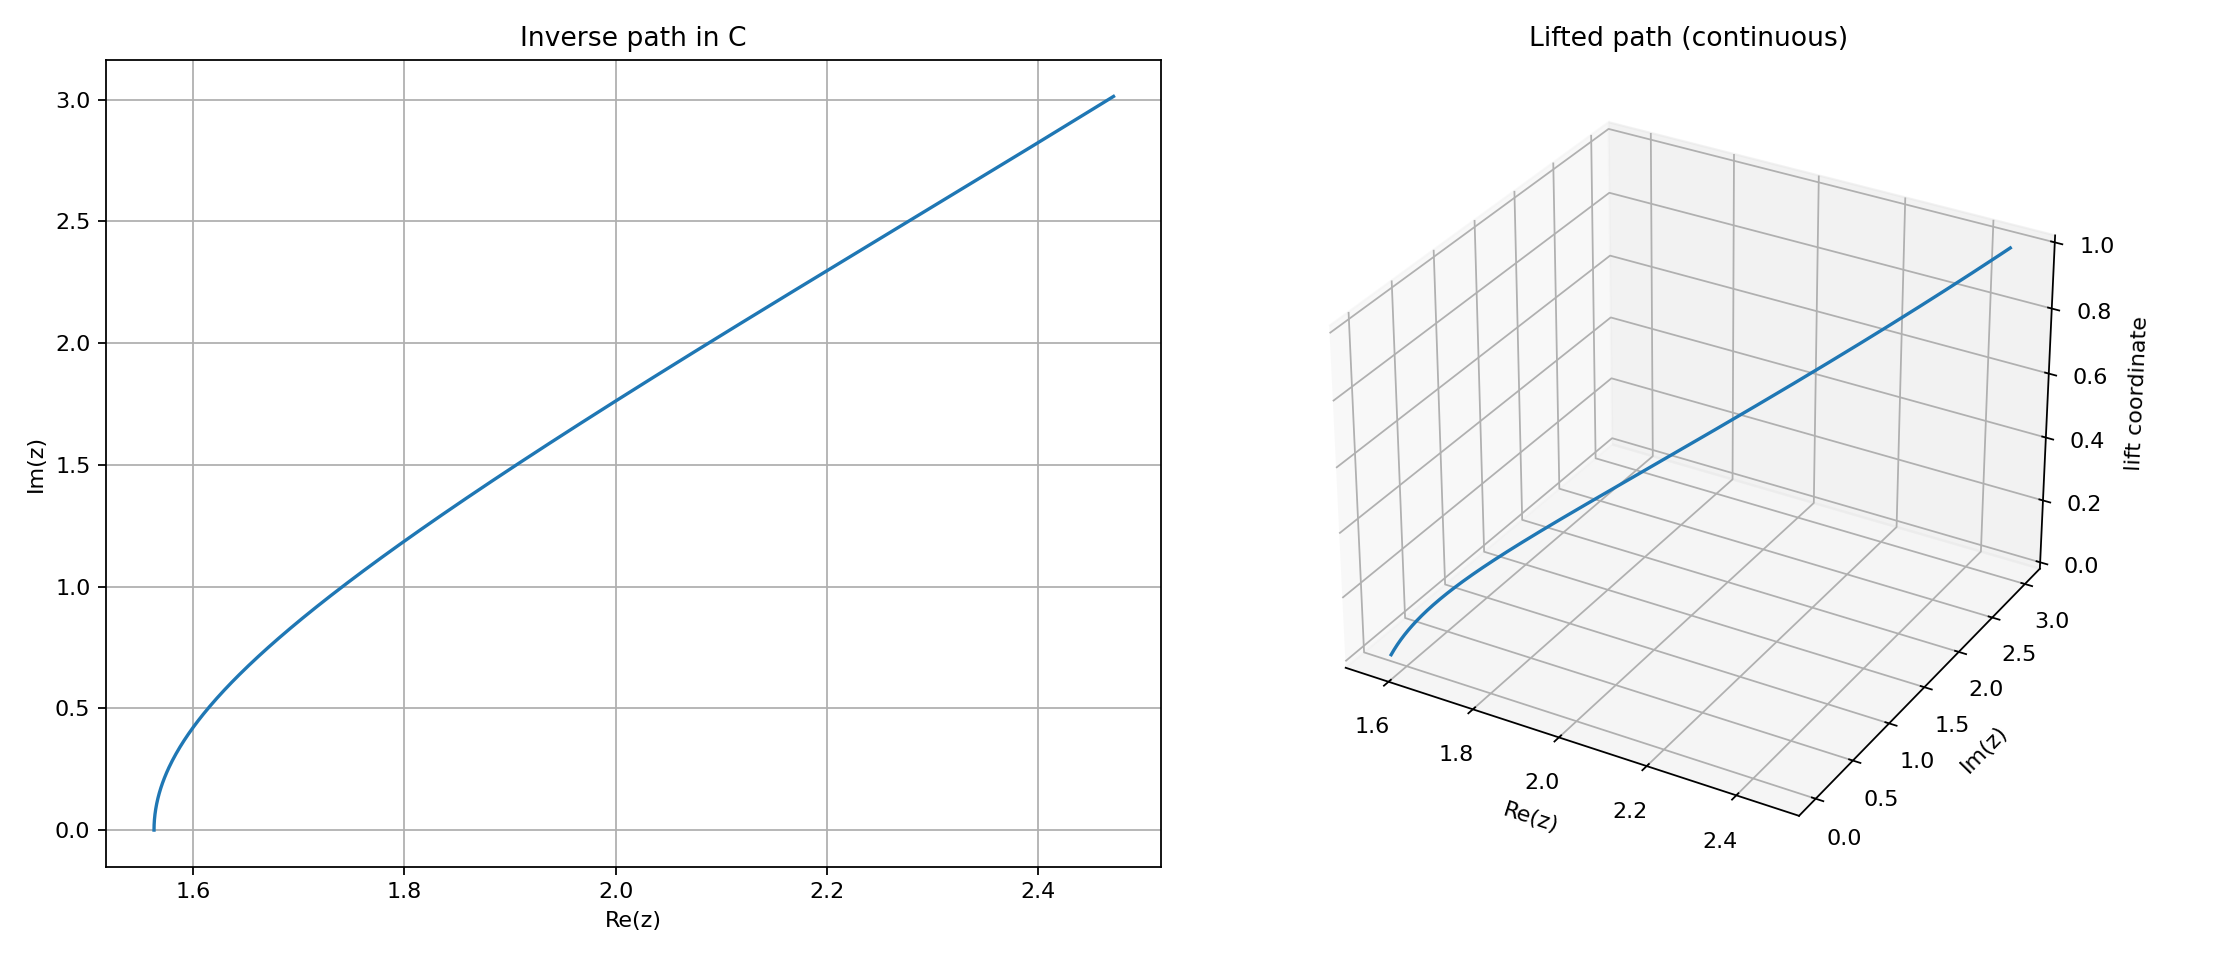
\includegraphics[width=0.85\textwidth]{inverse_z_to_z_demo.png}
  \caption{Experiment~1. Tracked inverse in $\mathbb{C}$ (left) and
    lifted view (right).}
\end{figure}

\begin{figure}[ht]
  \centering
  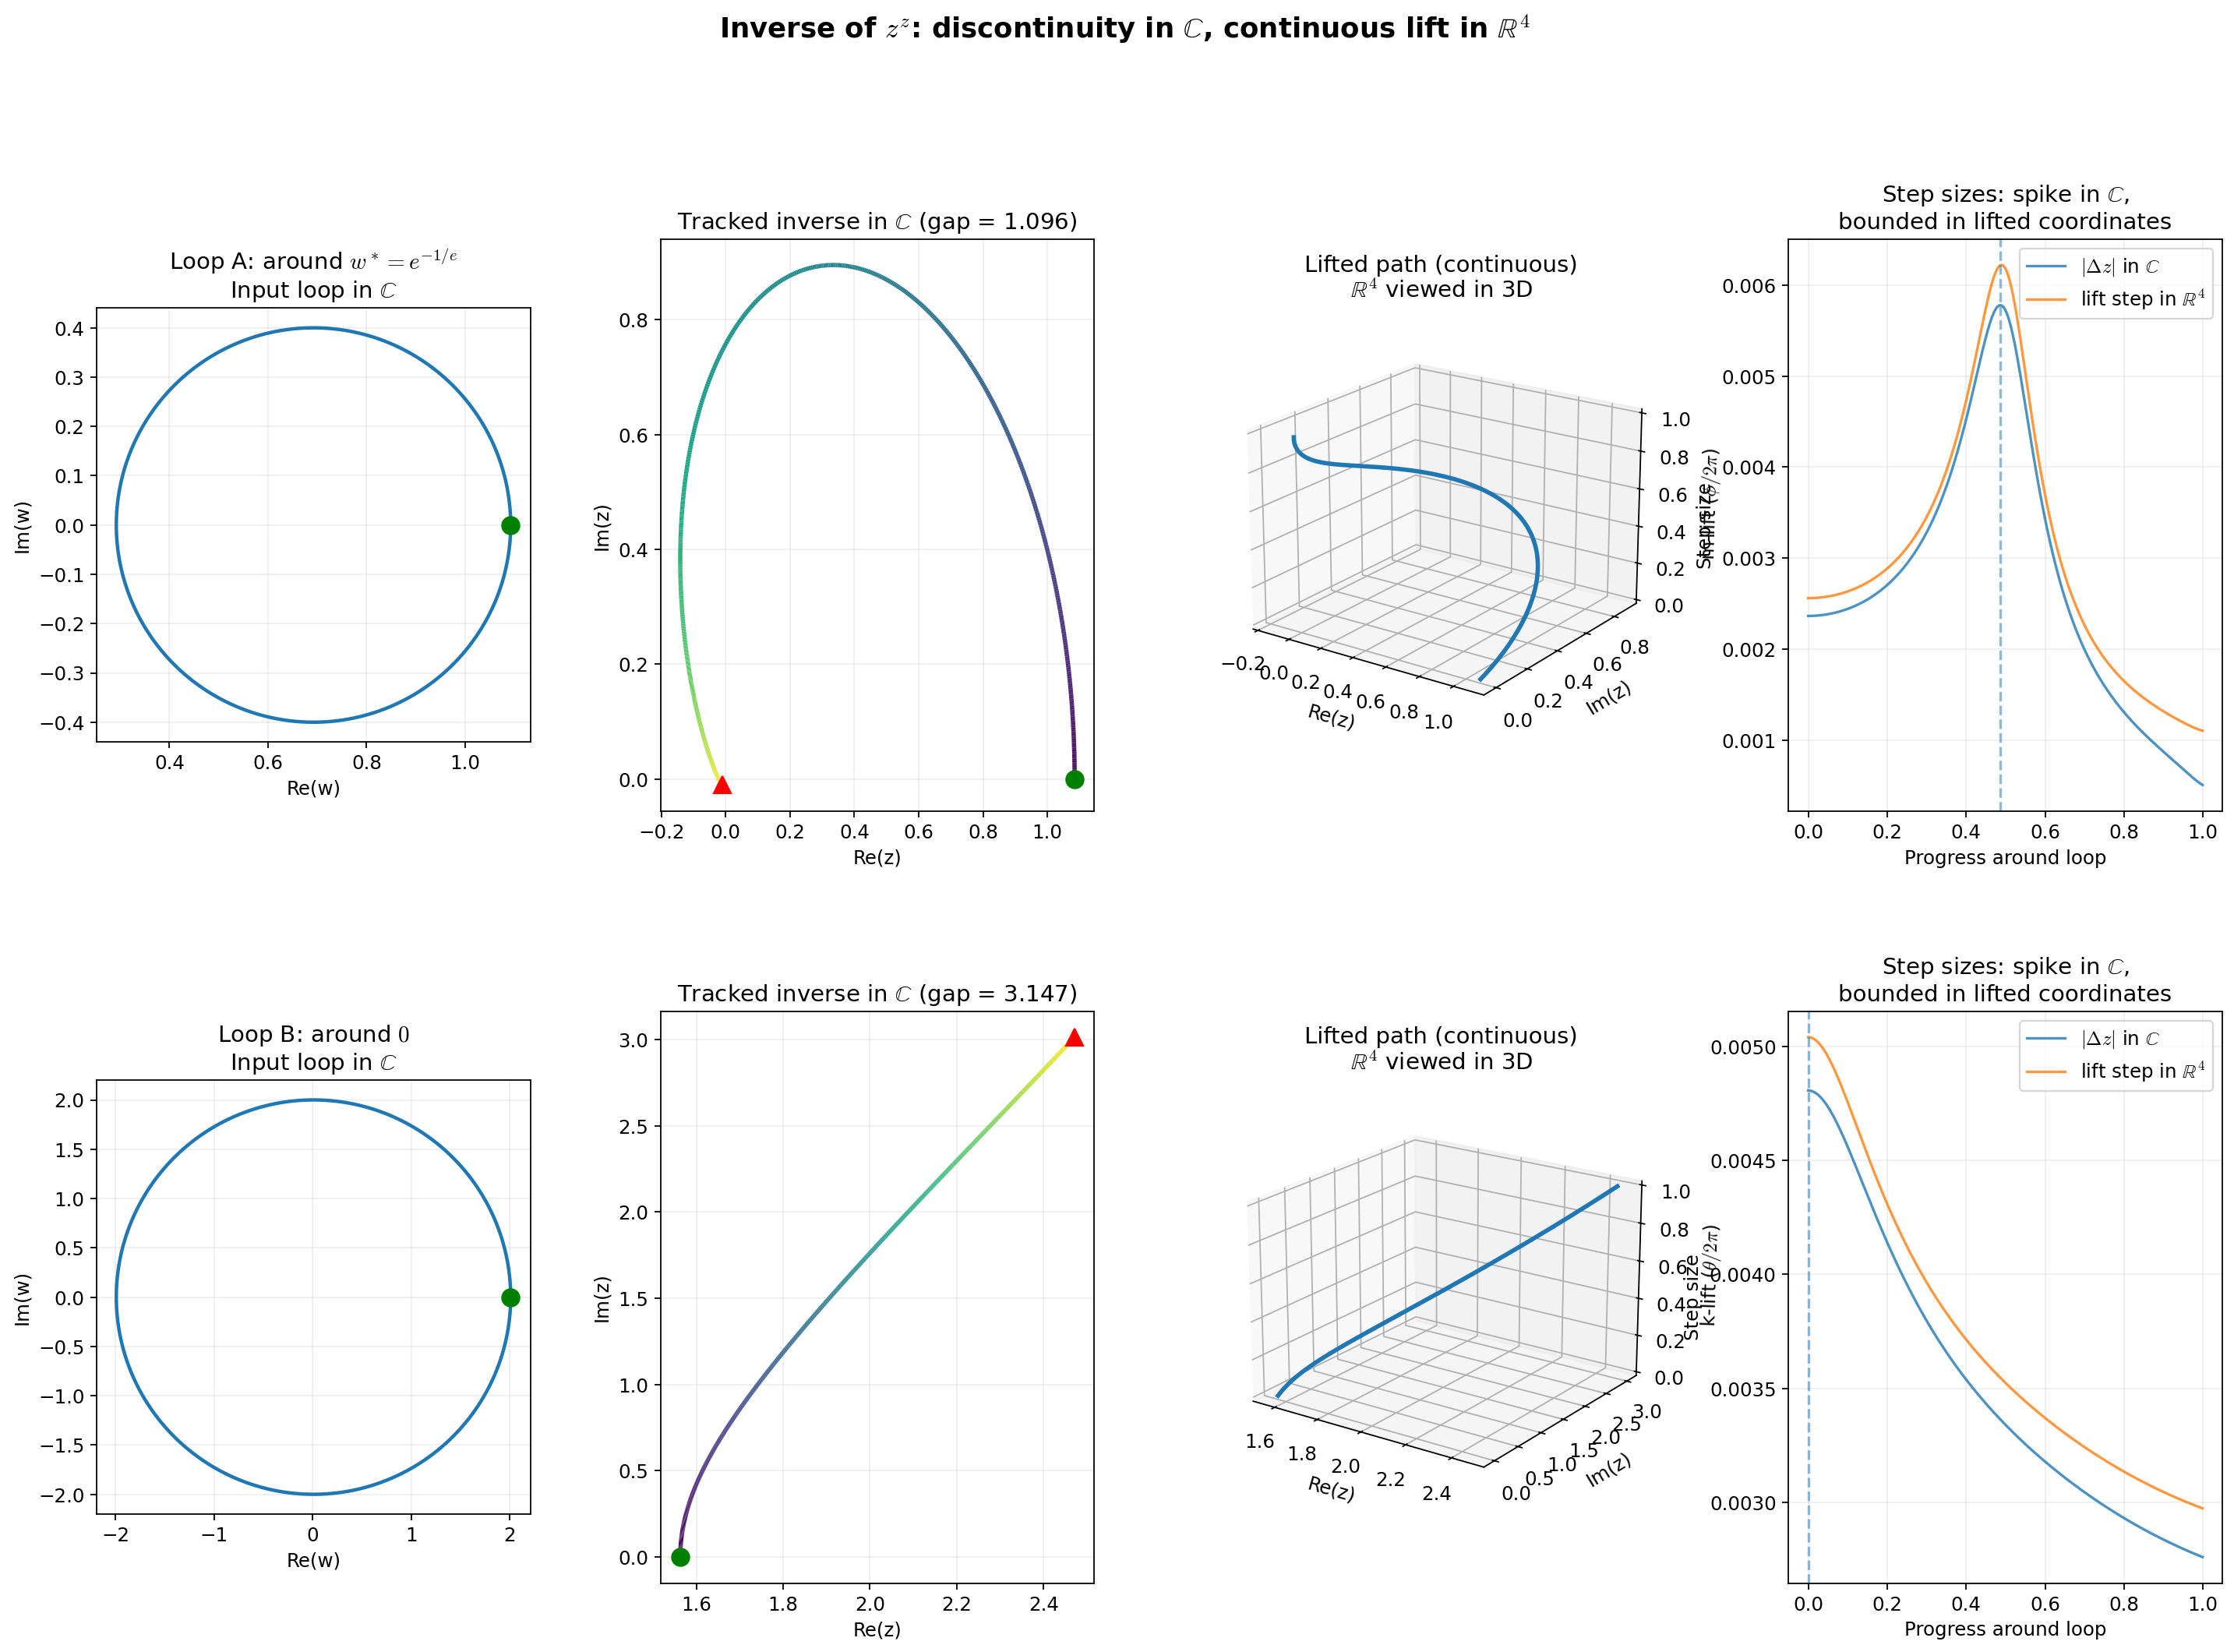
\includegraphics[width=0.95\textwidth]{fig_path_completion_lift.png}
  \caption{Experiment~2. Two-loop comparison with gaps and lift diagnostics.}
\end{figure}

\begin{figure}[ht]
  \centering
  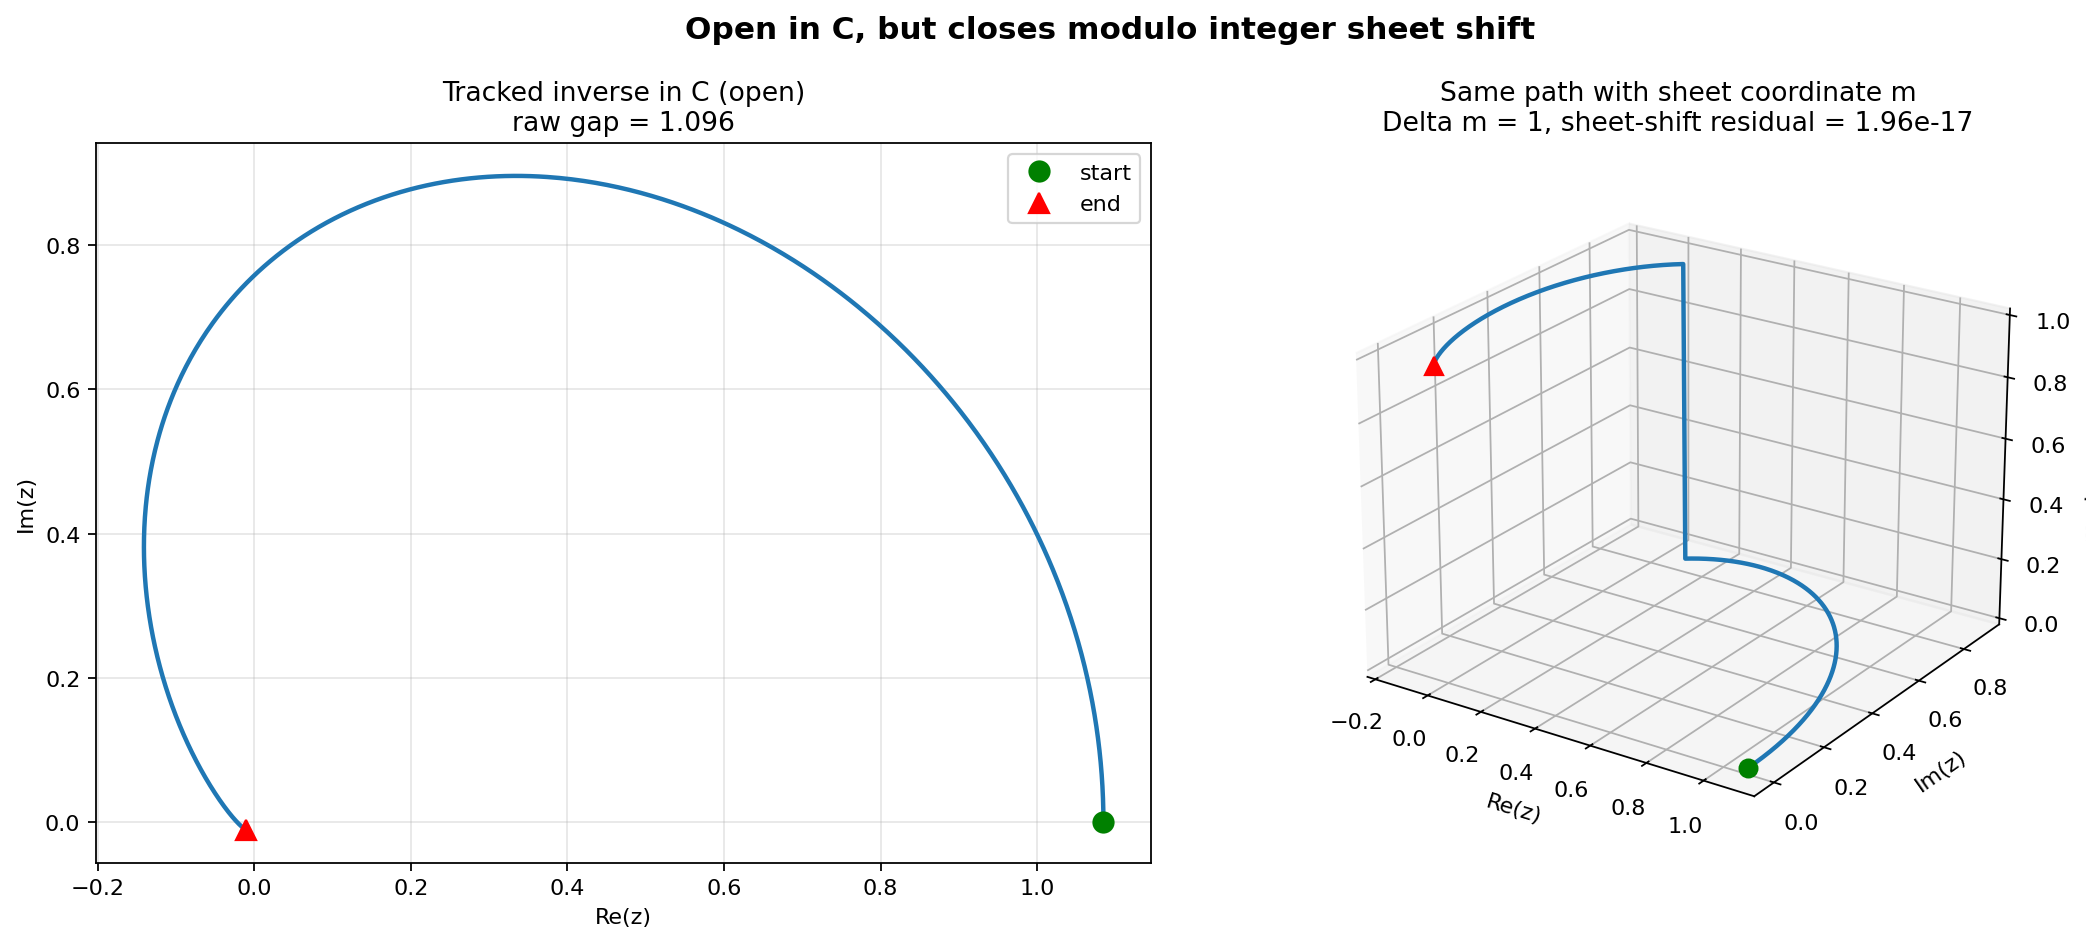
\includegraphics[width=0.85\textwidth]{fig_closure_mod_sheet_shift.png}
  \caption{Experiment~3. Open in $\mathbb{C}$, closed modulo sheet shift.}
\end{figure}

\begin{figure}[ht]
  \centering
  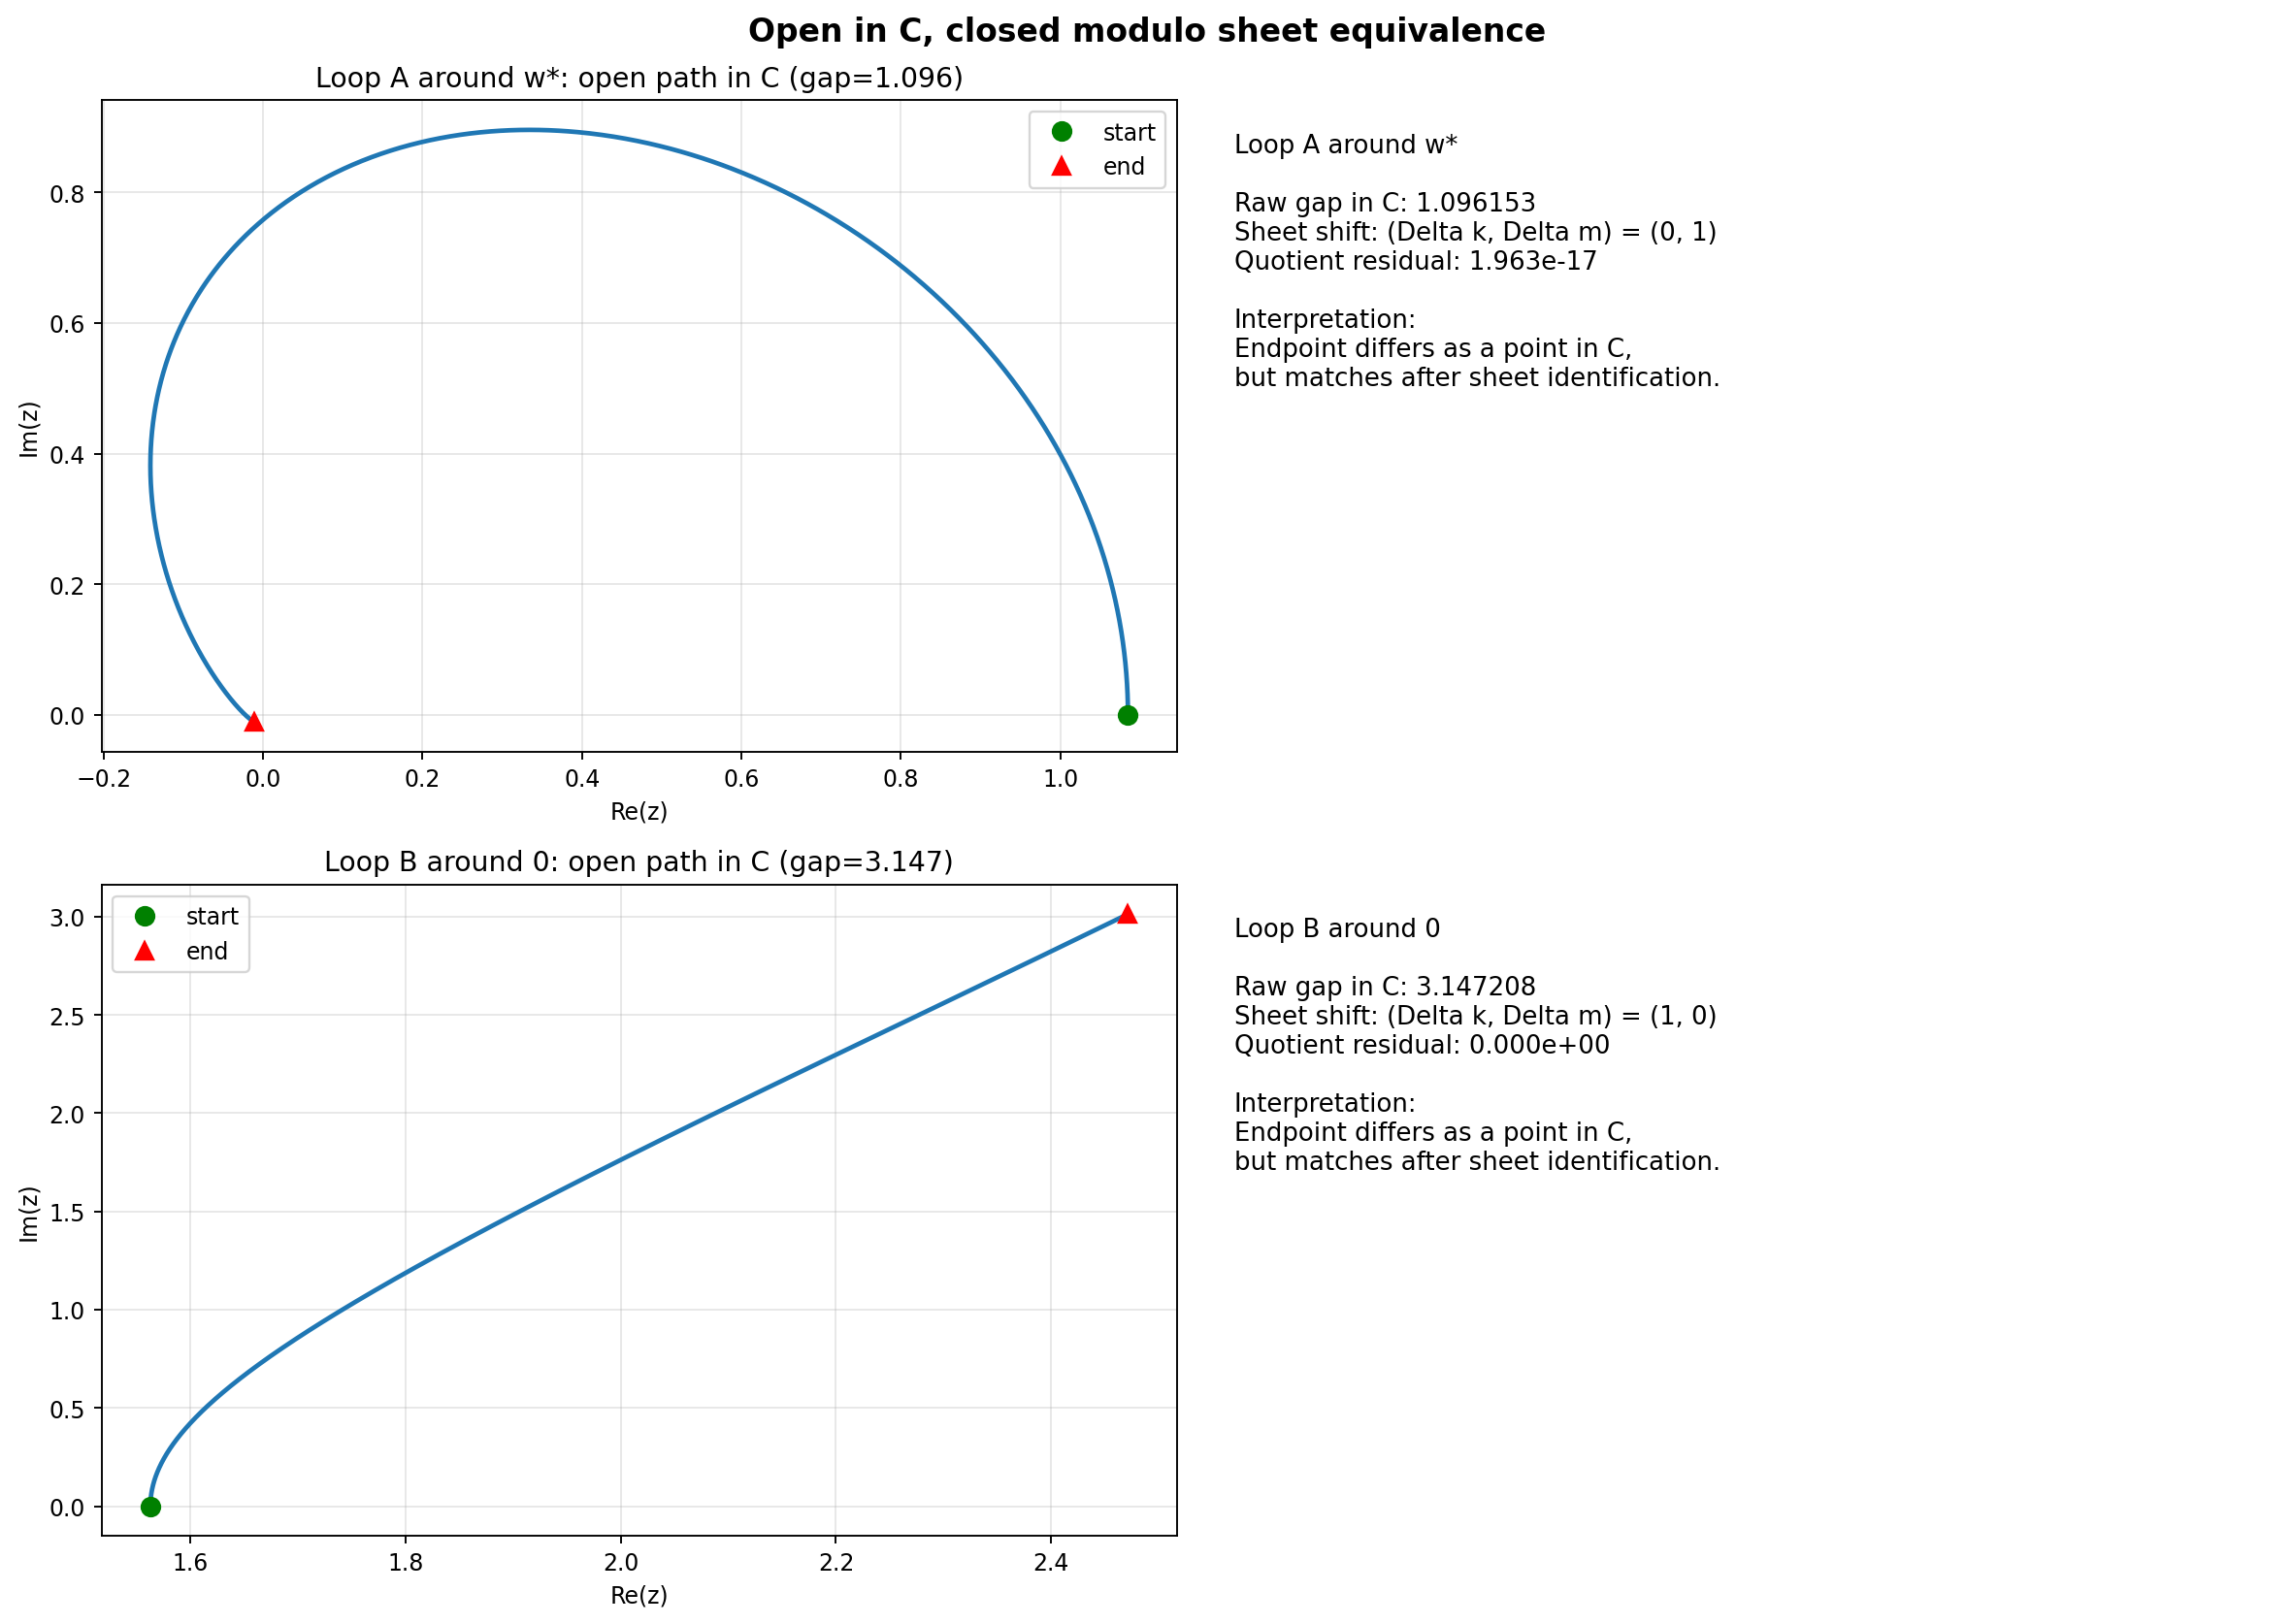
\includegraphics[width=0.85\textwidth]{fig_04_quotient_closure_demo.png}
  \caption{Experiment~4. Summary: quotient-closure with metrics.}
\end{figure}

\section{What This Does and Does Not Show}

\textbf{Shown:}
\begin{itemize}
\item Nontrivial monodromy: closed loops in $w$ produce open paths in $\mathbb{C}$.
\item Two independent integer branch generators: shifts $(0,1)$ and $(1,0)$.
\item Deck-action closure with machine-epsilon residuals.
\item Perfect stability across discretisation resolution.
\end{itemize}

\textbf{Not shown:}
\begin{itemize}
\item That monodromy of $z^z$ is multivalued is already known; these
      experiments demonstrate it, they do not discover it.
\item The experiments show $\mathbb{C}$ is insufficient, not that $4$
      dimensions are the \emph{minimum}. A lower bound needs a
      covering-space argument.
\item Only two loops are tested. The monodromy group could differ from
      $\mathbb{Z}\times\mathbb{Z}$; compositions and higher-winding tests
      are needed.
\item Nothing here tests quaternionic structure. The $\mathbb{H}$ aspect
      of the conjecture has zero computational support.
\item Nearest-neighbour continuation is heuristic (search radius
      $|dk|,|dm|\leq 2$, no formal error bound).
\end{itemize}

\end{document}
